% Block diagrams for the unit 6 slides, one tikzpicture per page.
%
% Built by make_figs.py (--blocks), which compiles this file and renders each
% page to <name>.png at 300 dpi.  The names are the "% fig:" comment above
% each picture, in page order; make_figs.py checks that the count matches.
%
% By hand:
%   pdflatex -shell-escape block_figs.tex
%   pdftocairo -png -r 300 -singlefile -f N -l N block_figs.pdf <name>
%
% Colours are the deck's (tools/build_timing_slides.py): teal for
% combinational logic, violet for registers and arrival times, amber for the
% critical path.  timing_figs.tex is the older, article-style source these
% were redrawn from.

\documentclass[tikz,border=4pt]{standalone}

\usepackage{amsmath}
\usepackage[scaled=0.92]{helvet}
\renewcommand{\familydefault}{\sfdefault}
\usepackage{../../styles/course}

\definecolor{violet}{HTML}{57068C}
\definecolor{tint}{HTML}{EEE6F3}
\definecolor{teal}{HTML}{00857C}
\definecolor{tealtint}{HTML}{DCEFEC}
\definecolor{amber}{HTML}{B4530F}
\definecolor{ink}{HTML}{262626}
\definecolor{muted}{HTML}{6E6E6E}

\tikzset{
  >=stealth,
  every picture/.style={line width=0.7pt, ink},
  blk/.style={draw=teal, fill=tealtint, text=ink, minimum height=0.9cm,
              minimum width=1.2cm, align=center, font=\small},
  op/.style={circle, draw=teal, fill=tealtint, text=ink, minimum size=6.5mm,
             inner sep=0pt},
  reg/.style={shape=register, draw=violet, fill=tint, minimum width=0.8cm,
              minimum height=1.6cm},
  mux/.style={blk, minimum width=1.0cm, minimum height=2.8cm},
  w/.style={->},
  % every node: the wire's name stays ink, not the wire's amber
  crit/.style={->, line width=2.2pt, amber, every node/.append style={text=ink}},
  critl/.style={-, line width=2.2pt, amber, every node/.append style={text=ink}},
  arr/.style={font=\small\bfseries, text=violet},
  sig/.style={font=\small\ttfamily},
  dly/.style={font=\scriptsize, text=muted},
  dot/.style={circle, fill=ink, inner sep=0pt, minimum size=3.5pt},
}

% A wire style that is "crit" in one picture and plain in another.
\newcommand{\cw}{w}

\begin{document}

% ----------------------------------------------------------------------
% Linear + ReLU in series.  #1..#4: the unknown interval written under the
% x, mult_out, add_out and y wires (empty for none).
% ----------------------------------------------------------------------
\newcommand{\reluseries}[4]{%
\begin{tikzpicture}
  \node[sig] (x) at (0,0) {x};
  \node[op] (m) at (1.7,0) {$\times$};
  \node[sig] (a) at (1.7,1.15) {a};
  \node[op] (ad) at (4.6,0) {$+$};
  \node[sig] (b) at (4.6,1.15) {b};
  \node[blk] (mx) at (7.4,0) {$\max\{u,0\}$};
  \node[sig] (y) at (9.7,0) {y};
  \draw[w] (x) -- node[arr, below=2pt] {#1} (m);
  \draw[w] (a) -- (m);
  \draw[w] (m) -- node[sig, above] {mult\_out} node[arr, below=2pt] {#2} (ad);
  \draw[w] (b) -- (ad);
  \draw[w] (ad) -- node[sig, above] {add\_out} node[arr, below=2pt] {#3} (mx);
  \draw[w] (mx) -- node[arr, below=2pt] {#4} (y);
\end{tikzpicture}}

% fig: relu_series
\reluseries{}{}{}{}
% fig: relu_s0
\reluseries{[0, 2]}{}{}{}
% fig: relu_s1
\reluseries{[0, 2]}{[0, 5]}{}{}
% fig: relu_s2
\reluseries{[0, 2]}{[0, 5]}{[0, 6.5]}{}
% fig: relu_s3
\reluseries{[0, 2]}{[0, 5]}{[0, 6.5]}{[0, 7.5]}

% ----------------------------------------------------------------------
% Multi-path: y = x*x + max(x, 0).  #1..#4: unknown intervals on x, xsq, r, y.
% ----------------------------------------------------------------------
\newcommand{\multipath}[4]{%
\begin{tikzpicture}
  \node[sig] (x) at (0,0) {x};
  \coordinate (s) at (0.9,0);
  \node[op] (m) at (2.4,0) {$\times$};
  \node[op] (ad) at (5.4,0) {$+$};
  \node[blk] (mx) at (3.4,-1.5) {$\max\{x,0\}$};
  \node[sig] (y) at (7.6,0) {y};
  \draw[-] (x) -- node[arr, above=2pt] {#1} (s);
  \node[dot] at (s) {};
  \draw[w] (s) -- (m);
  \node[dot] (s2) at (1.6,0) {};
  \draw[w] (s2) |- (1.9,0.65) -| (m.north);
  \draw[w] (s) |- (mx.west);
  \draw[w] (m) -- node[sig, above] {xsq} node[arr, below=2pt] {#2} (ad);
  \draw[w] (mx.east) -| node[sig, pos=0.75, right] {r} node[arr, pos=0.25, below=2pt] {#3} (ad.south);
  \draw[w] (ad) -- node[arr, above=2pt, pos=0.65] {#4} (y);
\end{tikzpicture}}

% fig: multipath
\multipath{}{}{}{}
% fig: multipath_s0
\multipath{[10, 12]}{}{}{}
% fig: multipath_s1
\multipath{[10, 12]}{[10, 15]}{[10, 13]}{}
% fig: multipath_s2
\multipath{[10, 12]}{[10, 15]}{[10, 13]}{[10, 16.5]}

% ----------------------------------------------------------------------
% fig: stable_block
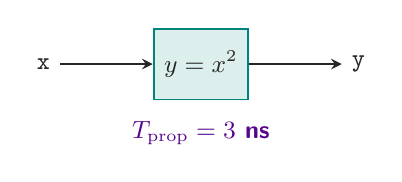
\begin{tikzpicture}
  \node[sig] (x) at (0,0) {x};
  \node[blk] (f) at (2.0,0) {$y = x^2$};
  \node[sig] (y) at (4.0,0) {y};
  \draw[w] (x) -- (f);
  \draw[w] (f) -- (y);
  \node[arr, below=4pt] at (f.south) {$T_{\mathrm{prop}} = 3$ ns};
\end{tikzpicture}

% ----------------------------------------------------------------------
% The conditional block: if (x > 0) z = f1(x); else z = f2(x); y = f3(z).
% #1: 1 to show delays and arrival times.  #2: 1 to mark the critical path.
% ----------------------------------------------------------------------
\newcommand{\condmux}[2]{%
\begin{tikzpicture}
  \ifnum#2=1 \tikzset{cp/.style={crit}, cpl/.style={critl}}%
  \else \tikzset{cp/.style={w}, cpl/.style={-}}\fi
  \ifnum#1=1 \tikzset{ar/.style={arr}}\else\tikzset{ar/.style={arr, opacity=0}}\fi
  \node[sig] (x) at (0,0) {x};
  \coordinate (s) at (1.0,0);
  \node[blk] (f1) at (3.0,1.0) {$f_1(x)$\ifnum#1=1\\[-1pt]{\scriptsize 4 ns}\fi};
  \node[blk] (f2) at (3.0,-0.7) {$f_2(x)$\ifnum#1=1\\[-1pt]{\scriptsize 2 ns}\fi};
  \node[mux] (mux) at (5.8,0.15) {mux\ifnum#1=1\\[-1pt]{\scriptsize 1 ns}\fi};
  \node[blk] (c) at (5.8,-2.45) {$x > 0$\ifnum#1=1\\[-1pt]{\scriptsize 0.5 ns}\fi};
  \node[blk] (f3) at (8.6,0.15) {$f_3(z)$\ifnum#1=1\\[-1pt]{\scriptsize 1.5 ns}\fi};
  \node[sig] (y) at (10.9,0.15) {y};
  \draw[cpl] (x) -- (s);
  \draw[cp] (s) |- (f1.west);
  \draw[w] (s) |- (f2.west);
  \draw[w] (s) |- (c.west);
  \draw[cp] (f1.east) -- node[ar, above] {4} (mux.west |- f1.east);
  \draw[w] (f2.east) -- node[ar, above] {2} (mux.west |- f2.east);
  \draw[w] (c) -- node[ar, right] {0.5} (mux.south);
  \draw[cp] (mux.east |- f3) -- node[sig, above] {z} node[ar, below] {4+1 = 5} (f3);
  \draw[cp] (f3) -- node[ar, below] {6.5} (y);
\end{tikzpicture}}

% fig: cond_mux
\condmux{0}{0}
% fig: mux_delays
\condmux{1}{0}
% fig: mux_critical
\condmux{1}{1}

% ----------------------------------------------------------------------
% fig: crit_example
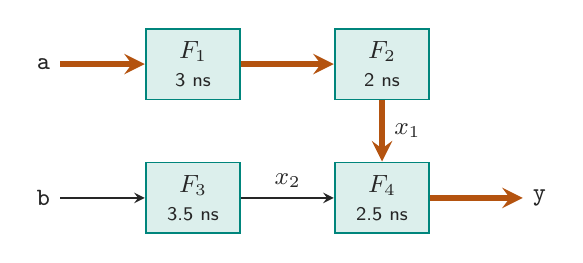
\begin{tikzpicture}
  \node[sig] (a) at (0,1.2) {a};
  \node[sig] (b) at (0,-0.5) {b};
  \node[blk] (f1) at (1.9,1.2) {$F_1$\\[-1pt]{\scriptsize 3 ns}};
  \node[blk] (f2) at (4.3,1.2) {$F_2$\\[-1pt]{\scriptsize 2 ns}};
  \node[blk] (f3) at (1.9,-0.5) {$F_3$\\[-1pt]{\scriptsize 3.5 ns}};
  \node[blk] (f4) at (4.3,-0.5) {$F_4$\\[-1pt]{\scriptsize 2.5 ns}};
  \node[sig] (y) at (6.3,-0.5) {y};
  \draw[crit] (a) -- (f1);
  \draw[crit] (f1) -- (f2);
  \draw[crit] (f2) -- node[sig, right] {$x_1$} (f4);
  \draw[w] (b) -- (f3);
  \draw[w] (f3) -- node[sig, above] {$x_2$} (f4);
  \draw[crit] (f4) -- (y);
\end{tikzpicture}

% ----------------------------------------------------------------------
% fig: adders_serial
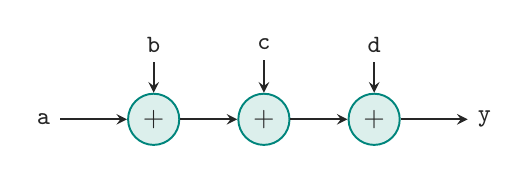
\begin{tikzpicture}
  \node[sig] (a) at (0,0) {a};
  \foreach \v/\x in {b/1.4, c/2.8, d/4.2} {
    \node[op] (p\v) at (\x,0) {$+$};
    \node[sig] (i\v) at (\x,0.95) {\v};
    \draw[w] (i\v) -- (p\v);
  }
  \node[sig] (y) at (5.6,0) {y};
  \draw[w] (a) -- (pb);
  \draw[w] (pb) -- (pc);
  \draw[w] (pc) -- (pd);
  \draw[w] (pd) -- (y);
\end{tikzpicture}

% fig: adders_parallel
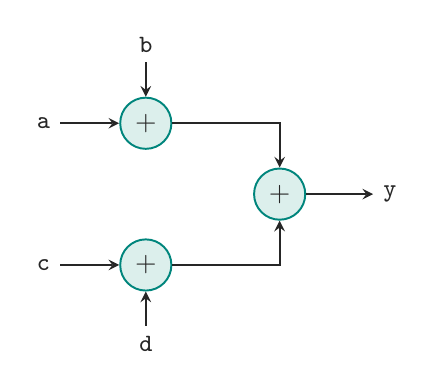
\begin{tikzpicture}
  \node[sig] (a) at (0,0.9) {a};
  \node[sig] (b) at (1.3,1.9) {b};
  \node[sig] (c) at (0,-0.9) {c};
  \node[sig] (d) at (1.3,-1.9) {d};
  \node[op] (p1) at (1.3,0.9) {$+$};
  \node[op] (p2) at (1.3,-0.9) {$+$};
  \node[op] (p3) at (3.0,0) {$+$};
  \node[sig] (y) at (4.4,0) {y};
  \draw[w] (a) -- (p1);
  \draw[w] (b) -- (p1);
  \draw[w] (c) -- (p2);
  \draw[w] (d) -- (p2);
  \draw[w] (p1) -| (p3);
  \draw[w] (p2) -| (p3);
  \draw[w] (p3) -- (y);
\end{tikzpicture}

% ----------------------------------------------------------------------
% fig: reg_loop
\begin{tikzpicture}
  \node[reg] (r) at (0,0) {};
  \node[sig] (clk) at (-1.4,-0.5) {clk};
  \draw[w] (clk) -- (r.clk);
  \node[blk] (f) at (2.4,0) {$f(x)$};
  \draw[w] (r.output) -- node[sig, above] {x} (f);
  \draw[-] (f.east) -- ++(0.6,0) |- (-0.9,1.4) node[sig, pos=0.75, above] {x\_next = f(x)};
  \draw[w] (-0.9,1.4) |- (r.input);
\end{tikzpicture}

% fig: dff
\begin{tikzpicture}
  \node[reg] (r) at (0,0) {};
  \node[sig] (d) at (-1.4,0) {D};
  \node[sig] (clk) at (-1.4,-0.5) {clk};
  \node[sig] (q) at (1.4,0) {Q};
  \draw[w] (d) -- (r.input);
  \draw[w] (clk) -- (r.clk);
  \draw[w] (r.output) -- (q);
\end{tikzpicture}

% ----------------------------------------------------------------------
% The two-variable system.  #1: 1 to show arrival times and the critical path.
% ----------------------------------------------------------------------
\newcommand{\twovar}[1]{%
\begin{tikzpicture}
  \ifnum#1=1 \tikzset{cp/.style={crit}, cpl/.style={critl}, ar/.style={arr}}%
  \else \tikzset{cp/.style={w}, cpl/.style={-}, ar/.style={arr, opacity=0}}\fi
  \node[sig] (x0) at (0,0) {$x_0$};
  \node[sig] (x1) at (0,-2.4) {$x_1$};
  \node[blk] (f1) at (1.9,0) {$f_1(x_0)$\ifnum#1=1\\[-1pt]{\scriptsize 1.8 ns}\fi};
  \node[blk] (f2) at (1.9,-1.2) {$f_2(x_1)$\ifnum#1=1\\[-1pt]{\scriptsize 2.2 ns}\fi};
  \node[blk] (f3) at (4.6,0) {$f_3(z_0,z_1)$\ifnum#1=1\\[-1pt]{\scriptsize 2.3 ns}\fi};
  \node[blk] (f4) at (4.6,-2.4) {$f_4(z_0,x_1)$\ifnum#1=1\\[-1pt]{\scriptsize 2.1 ns}\fi};
  \node[reg] (r0) at (8.4,0) {};
  \node[reg] (r1) at (8.4,-2.4) {};
  \draw[w] (x0) -- (f1);
  \draw[cpl] (x1) -- (0.6,-2.4);
  \draw[cp] (0.6,-2.4) |- (f2.west);
  \draw[w] (0.6,-2.4) -- (f4.west);
  \node[dot] at (0.6,-2.4) {};
  \draw[w] (f1) -- node[sig, above] {$z_0$} node[ar, below] {1.8} (f3);
  \draw[cp] (f2.east) -| node[sig, pos=0.3, above] {$z_1$} node[ar, pos=0.3, below] {2.2} (f3.south);
  \draw[w] (f1.east) ++(0.35,0) node[dot] {} |- (3.5,-1.95) -| ([xshift=-4mm]f4.north);
  \draw[cp] (f3) -- node[sig, above] {x\_next0} node[ar, below] {4.5} (r0.input);
  \draw[w] (f4) -- node[sig, above] {x\_next1} node[ar, below] {3.9} (r1.input);
  \draw[w] (r0.output) -- ++(0.6,0) node[right] {$x_0'$};
  \draw[w] (r1.output) -- ++(0.6,0) node[right] {$x_1'$};
\end{tikzpicture}}

% fig: twovar
\twovar{0}
% fig: twovar_crit
\twovar{1}

% ----------------------------------------------------------------------
% fig: sta_path
\begin{tikzpicture}
  \node[reg] (r0) at (0,0) {};
  \node[blk, minimum width=4.2cm, minimum height=1.2cm] (c) at (3.9,0)
    {combinational logic};
  \node[reg] (r1) at (7.8,0) {};
  \draw[w] (r0.output) -- (c);
  \draw[w] (c) -- (r1.input);
  \draw[-] (-0.9,-0.5) -- (r0.clk);
  \draw[-] (6.9,-0.5) -- (r1.clk);
  \node[sig, left] at (-0.9,-0.5) {clk};
  \draw[-] (-0.9,-0.5) -- (-0.9,-1.25) -| (6.9,-0.5);
  % timing brackets
  \def\yb{-1.95}
  \draw[|<->|, violet] (0.0,\yb) -- node[arr, below=2pt] {$T_{\mathrm{clk\text{-}Q}}$} (1.6,\yb);
  \draw[|<->|, teal] (1.6,\yb) -- node[font=\small\bfseries, text=teal, below=2pt] {$T_{\mathrm{PD}}$, combinational} (6.3,\yb);
  \draw[|<->|, amber] (6.3,\yb) -- node[font=\small\bfseries, text=amber, below=2pt] {$T_{\mathrm{setup}}$} (7.4,\yb);
  \draw[|<->|, ink] (0.0,-3.0) -- node[font=\small\bfseries, below=2pt] {$\le T_{\mathrm{clk}}$: one clock period} (7.4,-3.0);
\end{tikzpicture}

% ----------------------------------------------------------------------
% fig: delay_line
\begin{tikzpicture}
  \node[sig] (x) at (-1.5,0) {x};
  \node[reg] (r0) at (0,0) {};
  \node[reg] (r1) at (2.6,0) {};
  \node[sig] (y) at (4.1,0) {x1};
  \draw[w] (x) -- (r0.input);
  \draw[crit] (r0.output) -- node[sig, above, text=ink] {x0} (r1.input);
  \draw[w] (r1.output) -- (y);
  \node[font=\small, text=amber, align=center] at (1.3,-1.4) {short path: nothing between\\the registers to delay it};
\end{tikzpicture}

% ----------------------------------------------------------------------
% Synchronous linear + ReLU.  #1: 1 to show the arrival times.
% ----------------------------------------------------------------------
\newcommand{\relusync}[1]{%
\begin{tikzpicture}
  \ifnum#1=1 \tikzset{ar/.style={arr}}\else\tikzset{ar/.style={arr, opacity=0}}\fi
  \node[sig] (x) at (-1.4,0) {x};
  \node[reg] (rx) at (0,0) {};
  \node[sig] (a) at (0.4,1.9) {a};
  \node[reg, minimum height=1.2cm] (ra) at (1.6,1.9) {};
  \node[sig] (b) at (3.3,1.9) {b};
  \node[reg, minimum height=1.2cm] (rb) at (4.5,1.9) {};
  \node[op] (m) at (2.9,0) {$\times$};
  \node[op] (ad) at (5.8,0) {$+$};
  \node[blk] (mx) at (9.2,0) {$\max\{u,0\}$\ifnum#1=1\\[-1pt]{\scriptsize 1 ns}\fi};
  \node[sig] (y) at (11.4,0) {y};
  \draw[w] (x) -- (rx.input);
  \draw[w] (a) -- (ra.input);
  \draw[w] (b) -- (rb.input);
  \draw[w] (rx.output) -- node[sig, above] {xreg} node[ar, below] {0} (m);
  \draw[w] (ra.output) -| node[sig, pos=0.25, above] {areg} node[ar, pos=0.75, left] {0} (m.north);
  \draw[w] (rb.output) -| node[sig, pos=0.25, above] {breg} node[ar, pos=0.75, left] {0} (ad.north);
  \draw[w] (m) -- node[sig, above] {mult\_out} node[ar, below] {3} (ad);
  \draw[w] (ad) -- node[sig, above] {add\_out} node[ar, below] {3+1.5 = 4.5} (mx);
  \draw[w] (mx) -- node[ar, below] {5.5} (y);
  \ifnum#1=1
    \node[dly] at (2.9,-0.55) {3 ns};
    \node[dly] at (5.8,-0.55) {1.5 ns};
  \fi
\end{tikzpicture}}

% fig: relu_sync
\relusync{0}
% fig: relu_sync_sta
\relusync{1}

% ----------------------------------------------------------------------
% Quadratic y = w2 x^2 + w1 x + w0 in one cycle.  #1: 1 to mark path 1.
% ----------------------------------------------------------------------
\newcommand{\quadone}[1]{%
\begin{tikzpicture}
  \ifnum#1=1 \tikzset{cp/.style={crit}, cpl/.style={critl}}%
  \else \tikzset{cp/.style={w}, cpl/.style={-}}\fi
  \node[sig] (x) at (-1.4,0) {x};
  \node[reg] (r) at (0,0) {};
  \coordinate (s) at (1.5,0);
  \node[op] (m1) at (2.8,0) {$\times$};
  \node[op] (m2) at (4.6,0) {$\times$};
  \node[sig] (w2) at (4.6,1.0) {w2};
  \node[op] (a1) at (6.6,0) {$+$};
  \node[op] (a2) at (8.2,0) {$+$};
  \node[sig] (w0) at (8.2,1.0) {w0};
  \node[op] (m3) at (4.6,-1.4) {$\times$};
  \node[sig] (w1) at (4.6,-2.35) {w1};
  \node[sig] (y) at (9.6,0) {y};
  \draw[w] (x) -- (r.input);
  \draw[cpl] (r.output) -- node[sig, above, text=ink, pos=0.55] {x\_reg} (s);
  \node[dot] at (s) {};
  \draw[cp] (s) -- (m1);
  \node[dot] at (2.1,0) {};
  \draw[w] (2.1,0) |- (2.5,0.65) -| (m1.north);
  \draw[cp] (m1) -- node[sig, above, text=ink] {xsq} (m2);
  \draw[w] (w2) -- (m2);
  \draw[cp] (m2) -- node[sig, above, text=ink] {xsq\_w2} (a1);
  \draw[w] (s) |- (m3.west);
  \draw[w] (w1) -- (m3);
  \draw[w] (m3.east) -| node[sig, pos=0.25, below] {x\_w1} (a1.south);
  \draw[cp] (a1) -- (a2);
  \draw[w] (w0) -- (a2);
  \draw[cp] (a2) -- (y);
\end{tikzpicture}}

% fig: quad
\quadone{0}
% fig: quad_crit
\quadone{1}

% ----------------------------------------------------------------------
% The same quadratic over two cycles.  #1: 1 to mark the two 6.5 ns paths.
% ----------------------------------------------------------------------
\newcommand{\quadtwo}[1]{%
\begin{tikzpicture}
  \ifnum#1=1 \tikzset{cp/.style={crit}, cpl/.style={critl}}%
  \else \tikzset{cp/.style={w}, cpl/.style={-}}\fi
  \node[sig] (x) at (-1.4,0) {x};
  \node[reg] (r) at (0,0) {};
  \coordinate (s) at (1.5,0);
  \node[op] (m1) at (2.8,0) {$\times$};
  \node[reg] (rq) at (4.3,0) {};
  \node[op] (m2) at (5.9,0) {$\times$};
  \node[sig] (w2) at (5.9,1.0) {w2};
  \node[op] (ad) at (8.0,0) {$+$};
  \node[sig] (y) at (9.4,0) {y};
  \node[op] (m3) at (2.8,-1.7) {$\times$};
  \node[sig] (w1) at (2.8,-2.65) {w1};
  \node[op] (a0) at (4.0,-1.7) {$+$};
  \node[sig] (w0) at (4.0,-2.65) {w0};
  \node[reg] (rl) at (5.6,-1.7) {};
  \draw[w] (x) -- (r.input);
  \draw[cpl] (r.output) -- node[sig, above, text=ink, pos=0.55] {x\_reg} (s);
  \node[dot] at (s) {};
  \draw[w] (s) -- (m1);
  \node[dot] at (2.1,0) {};
  \draw[w] (2.1,0) |- (2.5,0.65) -| (m1.north);
  \draw[w] (m1) -- (rq.input);
  \draw[cp] (rq.output) -- node[sig, above, text=ink] {xsq} (m2);
  \draw[w] (w2) -- (m2);
  \draw[cp] (m2) -- (ad);
  \draw[cp] (s) |- (m3.west);
  \draw[w] (w1) -- (m3);
  \draw[cp] (m3) -- (a0);
  \draw[w] (w0) -- (a0);
  \draw[cp] (a0) -- (rl.input);
  \draw[w] (rl.output) -| node[sig, pos=0.25, above, text=ink] {lin\_term} (ad.south);
  \draw[cp] (ad) -- (y);
\end{tikzpicture}}

% fig: quad2
\quadtwo{0}
% fig: quad2_crit
\quadtwo{1}

\end{document}
